Während wir im vorherigen Kapitel Gradsequenzen als Stichproben einer Gradverteilung analysiert haben, möchten wir in diesem Kapitel konkrete Gradsequenzen als Charakterisierung eines Graphen verstehen.
Konkret möchten wir für eine gegebene Gradsequenz~$\degseq$ einen Graphen~$G$ erzeugen, der folgende Eigenschaften erfüllt:
\begin{enumerate}
    \item Graph~$G$ soll die Gradsequenz~$\degseq$ haben.
    \item Graph~$G$ soll einfach sein (d.h., keine Mehrfachkanten oder Schleifen haben).
    \item Graph~$G$ soll eine uniforme Stichprobe aus allen passenden Graphen sein.
\end{enumerate}

Im Folgenden werden wir eine Reihe von Ansätzen untersuchen.
Dabei wird sich zeigen, dass es einfach ist, wenn wir nur zwei Eigenschaften (d.h. 1\&2, 2\&3, oder 1\&3) erfüllen müssen.
Für eine allgemeine Gradsequenz~$\degseq$ ist es hingegen schwer allen drei Anforderungen gerechnet zu werden.

Bevor wir aber anfangen, sollten wir das \qq{Warum?} klären.
Es gibt zwei zentrale Motivationen Graphen mit allgemeinen Gradsequenzen erzeugen zu wollen:
\begin{itemize}
    \item
          Es handelt sich um einen Baustein für komplexere Generatoren.
          Ein bekanntes Beispiel ist das LFR-Benchmark~\cite{lancichinetti2008benchmark}, ein Zufallsgraph, um die Qualität von Community-Detection-Algorithmen zu messen.
          Hierfür werden Graphen erzeugt, von denen wir wissen, welche Knoten zu welchen Communities gehören.
          Der Generator erzeugt dafür parametrisierte Communities in Isolation und fügt diese dann zu seinem größeren Graphen zusammen.
          In beiden Schritten müssen Zufallsgraphen mit gegebenen Gradsequenzen erzeugt werden.

    \item
          In datengetriebenen Wissenschaften müssen wir regelmäßig die statistische Signifikanz von Beobachtungen messen.
          Oft bewerkstelligen wir diese durch Widerlegen einer Nullhypothese.

          Ein Beispiel in Network Science haben wir bereits gesehen:
          wir beobachteten Hub-Knoten, deren Grad wir nicht mit $\Gnp$ Graphen erklären konnten.
          Daraufhin schlugen wir das BA Modell vor.

          Wenig überraschend haben das $\Gnp$ und das BA Modell deutliche Unterschiede (z.B. sind selbst sehr dünne BA Graphen zusammenhängend).
          Egal welches Modell wir wählen, es führt immer zu einer Verzerrung in der Bewertung unserer Beobachtungen.

          Daher kommen nicht selten uniform zufällige und einfache Graphen, die dieselbe Gradsequenz wie das beobachtete Netz ausweisen, zum Einsatz.
\end{itemize}

\section{Configuration Model}
Ein Graph des Configuration Modells lässt sich wie folgt erzeugen.
Sei eine Gradsequenz~$\degseq = (d_1, \ldots, d_n)$ mit $\sum_i d_i$ gerade gegeben.
Dann legen wir für jedes $i$ genaue $d_i$ Bälle mit Aufdruck~$i$ in eine Urne.
Solange die Urne nicht leer ist, ziehen wir je zwei uniform zufällige Bälle ohne Zurücklegen.
Für jedes Paar mit Aufschrift $i$ und $j$ fügen wir die Kante $\set{i, j}$ in den Graph ein.
Per Konstruktion erhalten wir eine Ausgabe mit $m = (\sum_i d_i) / 2$ Kanten und $n$ Knoten.
Wir bezeichnen die Bälle als \emph{Halbkanten} oder \emph{stubs}, und mit \CMd die vom Configuration Model erzeugte Verteilung.

\medskip

\noindent
Prüfen wir kurz unser Lastenheft:
\begin{itemize}
    \item \emph{Graph~$G$ soll die Gradsequenz~$\degseq$ haben}.
          Das stimmt: per Konstruktion ist jede Knoten~$i$ genau $d_i$ mal vertreten.

    \item \emph{Graph~$G$ soll einfach sein (d.h., keine Mehrfachkanten oder Schleifen haben).}
          Das können wir nicht versprechen: niemand stoppt uns ein Paar $i = j$ zu ziehen, wenn $d_i > 1$.
          Analog kann es auch passieren, dass wir dasselbe Paar mehrfach ziehen.

    \item \emph{Graph~$G$ soll eine uniforme Stichprobe aus allen passenden Graphen sein.}
          Wenn wir zufällig einen einfachen Graphen produzieren, dann ist dieser uniform unter allen einfachen Graphen (siehe Übung).
\end{itemize}


\subsection{Effizientes Ziehen aus dem Configuration Model}
\begin{algorithm}[t]
    \KwIn{Gradsequenz $\degseq = (d_1, \ldots, d_n)$}
    \KwOut{Kantenarray $E$}

    \SetKwFunction{pushback}{pushBack}
    \SetKwFunction{popback}{popBack}

    \If{$\sum_i d_i \text{ ungerade}$}{
        breche mit Fehler ab\;
    }

    Allokiere leeres Array $U$ für Urne mit Kapazität $\sum_i d_i$\;
    \For{$1 \le i \le n$}{
        \For{$1 \le j \le d_i$}{
            $U.\pushback{i}$;
        }
    }

    Allokiere leeres Array $E$ für Kantenliste mit Kapazität $\sum_i d_i$\;
    \While{$U \neq \emptyset$}{
        $i \gets $ uniformer Index aus $\set{1, \ldots, |U|}$\;
        vertausche $U[i]$ und $U[|U|]$\;
        $x \gets U.\popback{}$\;
        \BlankLine
        $y$ analog gezogen wie $x$\;
        \BlankLine
        $E.\pushback{\set{x, y}}$\;
    }

    \caption{Linearzeit Generator das Configuration Model.}
    \label{alg:cm_einfach}
    \vspace{1em}
\end{algorithm}


Auf den ersten Blick benötigen wir erneut dynamisches gewichtetes Ziehen, um Knoten gewichtete nach ihrem Grad samplen zu können.
Derselbe Trick, den wir schon für BA Graphen gesehen haben, kann aber erneut angewendet werden.
Statt die $n$ veränderlichen Gewichte $d_1, \ldots, d_n$ abzuspeichern und daraus gewichtete zu ziehen, erzeugen wir ein Array mit $2m$ Einträgen (einen pro stub) und ziehen daraus uniform.
Der entsprechende Generator ist in \cref{alg:cm_einfach} skizziert.

Tatsächlich kennen wir aber einen sehr ähnlichen Algorithmus bereits, der sogar noch besser funktioniert.
Es handelt sich um den Fisher-Yates Shuffle: statt einer Urne und einer Kantenliste benötigen wir nur ein Array, das für jedes entnommene Element der Urne einen stub fixiert.
Wir können also das Configuration Model implementieren, in dem wir die Urne in eine zufällige Permutation bringen und dann je zwei benachbarte Einträge als Kante interpretieren.
Das hat den Vorteil, dass zufällige Permutation ein gut verstandenes Konzept sind und es auf diverse Plattformen effiziente Implementierungen gibt.

\begin{exercise}
    In der Praxis lässt sich dieser Ansatz sogar noch beschleunigen (besonders im parallelen Kontext).
    Wir partitionieren zunächst die Urne~$U[1..2m]$ anhand von Zufallsbits:
    am Anfang stehen alle Elemente für die wir eine 0 warfen, ans Ende kommen alle mit einer 1.
    Wir permutieren nun nur die größere der beiden Gruppen.
    Da partitionieren extrem schnell ist, ist der resultierende Algorithmus oft schneller.
    Zeige, dass wir einen Graphen des Configuration Models erhalten, wenn wir $U[i]$ und $U[2m - i + 1]$ als $i$-te Kante interpretieren.
\end{exercise}

\subsection{Graphische Gradsequenzen}
Wie wir im letzten Kapitel gesehen haben, kann das Configuration Model Mehrfachkanten und Eigenschleifen erzeugen.
Tatsächlich gibt es sogar Eingaben, für die sich das gar nicht vermeiden lässt.
Zum Beispiel: $\degseq = (2,)$, $\degseq = (2, 2)$, $\degseq = (3,3)$, oder $\degseq = (4, 1, 1)$.
Wir treffen daher folgende Definitionen:

\begin{definition}
    Sei $\gd$ die Menge aller einfache Graphen mit Gradsequenz~$\degseq$.
    Dann beschreibt $\Gd$ die uniforme Verteilung auf $\gd$.
\end{definition}

\begin{definition}
    Sei $\degseq$ eine Gradsequenz.
    Wir nennen $\degseq$ genau dann \emph{graphisch}, wenn $\gd \neq \emptyset$ (d.h., wenn es mindestens einen einfachen Graphen gibt, der $\degseq$ erfüllt).
\end{definition}

\noindent
Wir werden später zwei Charakterisierungen von \emph{graphischen} Gradsequenzen sehen.

\subsection{Erwartete Anzahl an Schleifen und Mehrfachkanten}\label{subsec:anzahl-illegaler-kanten}
Angenommen $\degseq$ ist graphisch.
Wie erhalten wir dann aus dem Configuration Model einen einfachen Graph?
Leider ist dies nicht immer exakt und effizient möglich.
Im Folgenden leiten wir aber her, dass die manchmal Situation gar nicht so schlimm ist.

Hierzu wechseln wir erneut von Gradsequenzen~\degseq{} zu Gradverteilungen.
Sei $p_d = n_d / n$ die Wahrscheinlichkeit, dass ein zufälliger Knoten Grad $d$ hat, wobei $n_d$ die Anzahl der Knoten in $\degseq$ mit Grad~$d$ beschreibt.
Die Wahl einer Gradverteilung erlaubt es uns nun beliebig große Graphen zu betrachten.
Wir verdeutlichen dies mit der Notation $\CMnd$.
In diesem Setting analysieren wir für große Knotenanzahl~$n$ die erwartete Anzahl von Mehrfachkanten $\expv{M_n}$ und Eigenschleifen~$\expv{S_n}$.

\begin{lemma}\label{lem:cm_anzahl_nicht_einfach}
    Sei $G \follows \CMnd$ ein von Configuration Model erzeugter Graph und $X$ ein zufälliger Grad mit $\prob{X = d} = p_d$.
    Wir bezeichnen mit $S_n$ die Anzahl der Eigenschleifen und mit $M_n$ die Anzahl der Mehrfachkanten.
    Dann gilt
    \begin{align}
        \expv{S_n} \approx c_n/2 \qquad \text{und} \qquad \expv{M_n} \le c_n^2 / 4,
    \end{align}
    wobei $c_n = (\expv{X^2} - \expv{X}) / \expv{X}$.
\end{lemma}

\begin{exercise}
    Seien $G_1$ und $G_2$ zwei Graphen mit gleicher Knoten- und Kantenanzahl.
    Beschreibe (qualitativ) zwei Gradverteilungen, s.d. wir für $G_1$ möglichst wenig kritische Kanten erwarten, während $G_2$ möglichst viele haben soll.
    Erkläre (qualitativ), weshalb $\expv{M_n} \propto \expv{S_n^2}$ plausible wirkt.
\end{exercise}

\begin{remark}
    Wie bereits in \cref{subsec:scaleinvariant} diskutiert, sind $\expv{X}$ und $\expv{X^2}$ das erste bzw. zweite Moment der Gradverteilung.
    Wir definieren also~$c_n$ über bekannte Größen von Wahrscheinlichkeitsverteilungen um es möglichst einfach anwenden zu können.
    Für den folgenden Beweis ist aber hilfreich, $c_n$ nachzurechnen.
    Für den Durchschnittsgrad wissen wir bereits
    \begin{align}
        \expv{X} & = \sum_{v_i \in V} \frac{d_i}{n} = \frac {2m}{n}.
    \end{align}

    \noindent
    Für das zweite Moment gilt gemäß seiner Definition
    \begin{align}
        \expv{X^2}
         & = \sum_{d=1}^{n-1} d^2 p_d
        = \sum_{d=1}^{n-1} d^2 (n_d / n)
        = \frac 1 n \underbrace{\sum_{d=1}^{n-1} n_d \cdot d^2}_\text{$n_d$ mal Grad $d$}
        = \frac 1 n \sum_{i=1}^n d_i^2.
    \end{align}

    \noindent
    Somit folgt $c_n$ als
    \begin{align}
        c_n
        = \frac{\expv{X^2} - \expv{X}}{\expv{X}}
        = \frac{ \frac 1 n \left(\sum_{i=1}^n d_i^2\right) - \frac 1 n \left(\sum_{i=1}^n d_i\right)}{\frac 1 n \sum_{i=1}^n d_i}
        = \sum_{i=1}^n \frac{d_i (d_i - 1)}{2m}.
    \end{align}
\end{remark}

\begin{proof}[Beweis von \cref{lem:cm_anzahl_nicht_einfach}]
    Sei $G= (V,E)$ mit $V = \set{v_1, \ldots, v_n}$.
    Dann bringt jeder Knoten $v_i \in V$ exakt $d_i$ Halbkanten $s_{1}^{(i)}, \ldots, s_{d_i}^{(i)}$ in die Urne ein.
    Wir nehmen an, dass diese unterscheidbar sind.

    \textbf{Schleifen. }
    Sei $I_{a,b}^{(i)}$ eine Indikatorvariable, die anzeigt, dass von Knoten $v_i$ die $a$-te und $b$-te Halbkante eine gemeinsame Kante (Eigenschleife!) bilden;
    hierzu betrachten wir nur $1\le a < b \le d_i$.
    Da die Halbkanten uniform zufällig gezogen werden und die Kantenreihenfolge irrelevant sind, gilt
    \begin{align}
        \prob{I_{a,b}^{(i)}} = \underbrace{\prob{I_{1,2}^{(i)}}}_\text{falls $d_i \ge 2$} = \frac{1}{2m - 1}.
    \end{align}

    \noindent
    Dann folgt die Schleifenanzahl als Summe der Erwartungswerte der Indikatorvariablen:
    \begin{align}
        \expv{S_n} & = \expv{\sum_{v_i \in V} \left( \sum_{1 \le a < b \le d_i} I_{a,b}^{(i)} \right)}                    \\
                   & = \sum_{v_i \in V}  \left( \sum_{1 \le a < b \le d_i} \textcolor{blue}{\expv{I_{a,b}^{(i)}}} \right) \\
                   & = \sum_{v_i \in V} \binom{d_i}{2} \textcolor{blue}{\prob{I_{1,2}^{(i)}}}                             \\
                   & = \frac 1 2 \sum_{v_i \in V} d_i (d_i - 1) \textcolor{blue}{\frac{1}{2m - 1}}                        \\
                   & \approx \frac 1 2 \sum_{v_i \in V} \frac{d_i (d_i - 1)}{2 m} = \frac{c_n}{2}
    \end{align}

    Beobachte, dass $I_{1,2}^{(i)}$ für Knoten~$v_i$ mit Grad $d_i <2$ nicht definiert ist.
    In diesem Fall ist aber auch $\binom{d_i}{2} = 0$; somit verzichten wir auf eine Ausnahmebehandlung.

    \textbf{Mehrfachkanten.}
    Die Beweisidee ist analog zur Schleifenanzahl, mit dem Unterschied, dass wir deutlich komplexere Indikatorvariablen benötigen.
    Wir nutzen $I^{(i,j)}_{a_1,b_1;a_2,b_2}$ um anzuzeigen, dass zwischen den Knoten $v_i$ und $v_j$ zwei Kanten existieren --- und zwar mit dem $a_1$-ten und $a_2$-ten Halbkanten von $v_i$ und den $b_1$-ten und $b_2$-ten Halbkanten von $v_j$.
    Es folgt:
    \begin{align}
        \prob{I^{(i,j)}_{a_1,b_1;a_2,b_2}} = \underbrace{\frac{1}{2m - 1}}_\text{erste Kante wie zuvor} \cdot \underbrace{\frac{1}{2m - 3}}_\text{Erste Kante fixiert zwei stubs}
    \end{align}

    Dies funktioniert gut für Doppelkanten; wenn im Graph eine Mehrfachkante mit höherer Multiplizität vorhanden ist, überschätzen wir diese aber (warum?).
    Daher leiten wir nur eine obere Schranke her.
    Beachte, dass die zwei Approximationen die Schranke eigentlich reduzieren, jedoch asymptotisch irrelevant sind:
    \begin{align}
        \expv{M_n}
         & \le \sum_{v_i, v_j \in V\colon i \textcolor{red!50!black}{\le} j} \left[ \sum_{1 \le a_1 \textcolor{green}{<} a_2 \le d_i} \left( \sum_{1 \le b_1 \textcolor{red}{\ne} b_2 \le d_j} \prob{I^{(i,j)}_{a_1,b_1;a_2,b_2}} \right) \right] \\
         & \approx \underbrace{\textcolor{red!50!black}{\frac 1 2}}_\text{Approx.} \sum_{v_i, v_j \in V} \left[ \textcolor{green}{\binom{d_i}{2}} \textcolor{red}{2\binom{d_j}{2}} \frac{1}{(2m - 1)(2m - 3)}   \right]                           \\
         & \approx \sum_{v_i, v_j \in V} \left[ \binom{d_i}{2} \binom{d_j}{2} \frac{1}{(2m)(2m)}   \right]                                                                                                                                        \\
         & = \left[ \frac{1}{2} \sum_{v_i \in V} \frac{d_i (d_i - 1)}{2m}  \right] \left[ \frac{1}{2} \sum_{v_j \in V} \frac{d_j (d_j - 1)}{2m} \right]
        = \frac{c_n^2}{4} \qedhere
    \end{align}
\end{proof}

Beobachte, \aside{Erased Configuration Model} dass für Gradverteilung mit endlichen ersten und zweiten Moment, $c_n$ für $n \to \infty$ konvergiert.
Ein Beispiel hierfür sind etwa reguläre Graphen.
In diesem Fall ergibt sich eine erwartete konstante Anzahl an illegalen Kanten, die für $n \to \infty$ eine immer kleinere Rolle spielen.
Ein probates Mittel ist es daher Eigenschleifen zu entfernen und von jeder $k$-fachen Mehrfachkante $k{-}1$ Exemplare zu löschen.
Man spricht vom sogenannten \emph{Erased Configuration Model}.

Während für Gradverteilungen mit $c_n = \Oh{1}$ das \emph{Erased Configuration Model} kaum Einfluss auf die Gradsequenz des Graphen hat, ist das für Graphen mit $c_n = \omega(1)$ nicht immer der Fall.
Insbesondere skalenfrei Powerlaw Verteilungen sind notorisch schwierig.
Dies liegt unter anderem daran, dass illegale Kanten häufiger auftreten und sich zudem um Hubs herum konzentrieren.
Das \emph{Erased Configuration Model} hat daher einen Bias den Grad von Knoten mit vielen Nachbarn besonders stark abzusenken;
dies wiederum hat signifikante Auswirkungen auf die Graphstruktur (siehe z.B. \cite{DBLP:journals/snam/SchlauchHZ15}).
Wir werden später Techniken diskutieren, die illegale Kanten entfernen können, ohne dabei die Gradsequenz zu verändern.

\subsection{Ans Gute glauben und das Schlechte ablehnen}
In \cref{subsec:anzahl-illegaler-kanten} zeigten wir, dass der Anteil illegaler Kanten bei gutmütigen Verteilungen zu vernachlässigen ist.
Wir können aber noch einen Schritt weiter gehen, und uns fragen, mit welcher Wahrscheinlichkeit sehen wir \emph{gar keine} nicht-einfachen Kanten?

Mit einer sorgsamen Analyse können wir zeigen, dass für $c_n = \Oh{1}$ und $n \to \infty$ die Größen $S_n$ und $M_n$ gegen unabhängige Poisson-verteilte Zufallsvariablen mit $\lambda = c_n/2$ bzw. $\lambda = c_n^2/4$ konvergieren.
Das wiederum führt direkt zu folgendem Satz.

\begin{theorem}\label{thm:einfaches_cm}
    Sei $G \follows \CMnd$. Dann ist die Wahrscheinlichkeit, dass $G$ einfach ist
    \begin{align}
        \prob{\text{$G$ ist einfach}} = \exp\left(-\frac{c_n}{2}\right)\exp\left(-\frac{c_n^2}{4}\right)(1 + o(1)). \hspace{2cm}\qedhere
    \end{align}
\end{theorem}

Beachte, dass wir in den vorherigen Kapiteln typischerweise exponentielle Schranken für die Fehlerwahrscheinlichkeit gezeigt haben.
\Cref{thm:einfaches_cm} hingegen beschränkt die Erfolgswahrscheinlichkeit.
Für $c_n \ggg 0$ ist das also ein katastrophales Resultat.

Selbst für eigentlich gutmütige reguläre Graphen kommen wir schnell an unsere Grenzen.
Wenn wir aber einen sehr kleinen Grad, etwa $r = \alpha 2 \sqrt{\log{n}}$, wählen, ergibt sich aber wenigstens noch eine erwartete polynomielle Laufzeit:
\begin{align}
    c_n = \frac{\expv{X^2} - \expv{X}}{\expv{X}} = \frac{r^2 - r}{r} \approx r = \alpha\sqrt{\log n}
\end{align}

\noindent
Somit ergibt sich eine Erfolgswahrscheinlichkeit von
\begin{align}
    \prob{\text{$G$ ist einfach}}
    = \exp\left(-\frac{c_n}{2}\right)\exp\left(-\frac{c_n^2}{4}\right)(1 + o(1))
    = \Omega\left(\frac{1}{n^{2\alpha}}\right).
\end{align}

Wenn wir solange Graphen produzieren, bis wir zufällig einen einfachen Graph erhalten haben, reichen also in Erwartung $\Oh{n^{2\alpha}}$ Versuche.
Tatsächlich handelt es sich hierbei dann auch um ein uniformes zufälliges Sample aus $\gd$ (siehe Rejection Sampling).
Da jeder Graph in Zeit $\Oh{rn}$ erzeugt werden kann, ergibt sich also ein Generator mit polynomieller Laufzeit.

\subsection{Einzelne Kanten zurückweisen}
Obwohl uns \cref{lem:cm_anzahl_nicht_einfach} verspricht, dass für viele Gradverteilungen der Anteil der illegalen Kanten asymptotisch insignifikant ist, zeigt uns die Diskussion, dass es oft relativ unwahrscheinlich ist, einen vollständig einfachen Graph zu erhalten.
Das liegt schlicht daran, dass eine einzige illegale Kante unter $2m$ Kanten, zum Misserfolg führt.
Die Idee liegt auf der Hand:

Während wir die Kanten iterativ aus der Urne entnehmen, prüfen wir, ob die gezogene Kante legal ist.
Falls nicht, legen wir die beiden Bälle zurück in die Urne und versuchen es erneut.
Leider können wir hierbei \qq{stecken bleiben}.
Als Extrembeispiel betrachten wir für großes $k \ggg 0$ die folgende Gradsequenz über $n = k + 1$ Knoten:
\begin{align}
    \degseq = \left(
    \underbrace{k-1, k-1, \ldots, k-1}_\text{$k-1$ mal},
    \underbrace{k}_\text{Knoten $u$},
    \underbrace{1}_\text{Knoten $v$}
    \right)
\end{align}

Hierbei handelt es sich um eine sog. Threshold Sequenz --- eine Gradsequenz bei denen alle einfache Graph isomorph sind (d.h. wenn wir die Knotenindizes löschen sind alle Graphen identisch).
Die hier beschriebene Sequenz erzeugt einen Graph mit einer Clique aus $k$ Knoten, wobei einer der Knoten~$u$ noch zu Knoten~$v$ verbunden ist.

Das Problem besteht nun darin, dass das Blatt~$v$ genau zu Knoten~$u$ verbunden sein muss.
Die Wahrscheinlichkeit, dass just diese Kante erzeugt wird skaliert aber grob mit $1/n$.
Sobald wir das Blatt~$v$ mit einem anderen Knoten~$u' \ne u$ verbunden haben, gibt es keine Möglichkeit die verbleibende Grade nur mit einfachen Kanten zu verteilen.
Es bleibt also grob 1 Versuch aus $\Oh{n}$ nicht stecken.

Wir betrachten daher einen anderen Zufallsgraph.

\section{Chung-Lu Graphen}
Das Kernproblem einzelne Kanten im Configuration Model zurückzuweisen besteht darin, dass jede gezogene Kante einen Effekt auf folgende Kanten hat ---
einfach weil wir ohne Zurücklegen ziehen und jede eingefügte Kante zwei Bälle aus der Urne entfernt.
Das Chung-Lu Modells hat strukturelle Ähnlichkeiten zum Configuration Model, umgeht aber genaue diese Schwäche.

Die Eingabe des Chung-Lu Modells besteht aus einem Vektor $w = (w_1, \ldots, w_n) \in \mathbb{R}_{>0}^n$, der die Funktion einer Gradverteilung übernimmt und nicht normiert sein muss.
Daher ist auch die Wahl $w = \degseq$ nicht unüblich.
Es wird dann ein Graph mit $n$ Knoten erzeugt und jede Kante~$\set{v_i,v_j}$ unabhängig mit Wahrscheinlich $p_{i,j}$ eingefügt.
Es gilt
\begin{align}
    \prob{\set{v_i,v_j} \in E} = p_{i,j} := \frac{w_iw_j}{\sigma} \qquad \text{mit} \qquad \sigma = \sum_{v \in V} w_v
\end{align}

Per Definition kann es also keine Mehrfachkanten geben.
In der Analyse des Chung-Lu Modells werden in der Regel Eigenschleife erlaubt, um Sonderfälle zu vermeiden.
In praktischen Implementierung ist es aber trivial diese zu verbieten.

Betrachten wir zunächst den erwarteten Grad~\expv{\deg{v_i}}:
\begin{align}
    \expv{\deg{v_i}} & = \sum_{v_j \in V} p_{i,j} = \sum_{v_j \in V} \frac{w_iw_j}{\sigma}      \\
                     & =w_i \cdot \frac{1}{\sigma} \underbrace{\sum_{v_j \in V} w_j}_{= \sigma} \\
                     & = w_i
\end{align}

Das Gewicht~$w_i$ eines Knotens~$v_i$ entspricht also seinem erwarteten Grad.
Bei der Wahl von $w$ müssen wir jedoch dafür sorgen, dass für alle $i, j$ der Parameter~$p_{i,j} \le 1$ sich als Wahrscheinlichkeit eignet.
Beachte, dass das gilt (weshalb?):
\begin{align}
    \max_{i,\textcolor{red}{j}} \set{p_{i,\textcolor{red}{j}}} \le \max_{i}\set{p_{i,\textcolor{red}{i}}}
\end{align}

Daher können wir durch Beschränkung der \qq{Diagonaleinträge} gleichzeitig alle $p_{i,j}$ nach oben beschränken.
Um nun sicherzustellen, dass alle $p_{i,j} \le 1$ wird oft gefordert:
\begin{align}
    \max_i{\left(w_i^2\right)} \le \sigma
    \qquad \Leftrightarrow \qquad \max_i{\left(\frac{w_iw_i}{\sigma}\right)} \le 1
    \qquad \Leftrightarrow \qquad \max_i{\left(p_{ii}\right)} \le 1.
\end{align}

Eine Alternative besteht darin, die Definition von $p_{i,j}$ um eine explizite obere Schranke zu erweitern:
\begin{align}
    p'_{i,j} = \min(1, \frac{w_iw_j}{\sigma})
\end{align}

Von Anwenderseite ist $p'_{i,j}$ bequemer, da $w$ weniger Restriktionen unterliegt;
die Analyse des Modells wird aber unhandlicher.
Daher nutzen wir im Folgenden die ursprüngliche Definition und gehen davon aus, dass $w$ korrekt beschränkt ist.

Bevor wir uns effiziente Generatoren für das Chung-Lu Modell ansehen, diskutieren wir uns zunächst einige allgemeine Sampling-Techniken, die hierfür nützlich sein werden.

\subsection{Rejection Sampling}
Im Folgenden verallgemeinern wird die sog. Verwerfungsmethode (rejection sampling), die wir bereits in einer sehr einfachen Ausprägung beim Ziehen ohne Zurücklegen und Generieren einfacher Graphen genutzt haben.
Damals war die Kernidee jedes Mal etwa:
\floatmarginfigure{
    \begin{tikzpicture}
        \node[draw, minimum width=4cm, minimum height=4cm] {};

        \foreach \x in {-18, -16, ..., 18} {
                \foreach \y in {-18, -16, ..., 18} {
                        \node[circle, inner sep=0, minimum width=0.5mm, fill] at (\x mm, \y mm) {};
                    }
            }
        \node[fill=blue, opacity=0.2, cloud, minimum width=3.8cm, minimum height=2.5cm] (c) at (0,0) {};
        \node[draw, cloud, minimum width=3.8cm, minimum height=2.5cm] (c) at (0,0) {Ziel};
    \end{tikzpicture}
    \caption{Rejection Sampling für Uniforme Verteilung}
    \label{fig:rejection-uniform}
}
Wir nutzen einen stochastischen Prozess, der uns Vorschläge unterbreitet (proposal distribution).
Dieser Prozess hatte bereits die gewünschte Verteilung, lieferte aber u.\,U. Vorschläge, die wir kategorisch ablehnen mussten;
beim $\Gnm$-Modell mussten wir bereits gezogene Kanten zurückweisen.
Beim BA-Modell waren es Knoten, zu denen wir bereits verbunden sind, und beim Configuration Model verwarfen wir nicht einfache Graphen.
Nach dem Ablehnen unerwünschter Element erhielten wir dann die Zielverteilung (target distribution) automatisch.

\Cref{fig:rejection-uniform} veranschaulicht diese Idee.
Die proposal distribution entspricht der uniformen Verteilung in der Box (visualisiert durch das reguläre Gitter).
Die Zielverteilung ist ebenfalls uniform -- allerdings über einer eingeschränkten Grundgesamtheit.
Das Gitter ist auch auf dieser uniform verteilt.

Ein weiteres Beispiel ist ein normaler Spielwürfel mit sechs gleich wahrscheinlichen Seiten, die von $1$ bis $6$ beschriftet sind.
Wir können mit diesem Würfel uniform aus \set{1,2,3,4,5} ziehen:
Falls eine Sechs gewürfelt wird, verwerfen wir diese und versuchen es erneut.
In Erwartung benötigen wir $6/5$ Versuche, um ein Ergebnis zu produzieren.

Die Verwerfungsmethode ist aber mächtiger -- es muss nicht immer ganz oder gar nicht sein.
Sie eignet sich auch, um die Wahrscheinlichkeit in einzelnen Bereichen anzuheben bzw. abzusenken.

Angenommen, wir möchten die Zielverteilung~$T$ mit $t\colon \Omega \to [0, 1]$ erzeugen.
Dann benötigen wir einen Generator für die Verteilung~$P$, der einen Vorschlag mit Wahrscheinlichkeitsverteilung $p\colon \Omega \to [0, 1]$ erzeugt.
Wir gehen davon aus, dass mindestens ein $x \in \Omega$ existiert, s.\,d. $t(x) \ne p(x)$ -- sonst sind die Verteilungen identisch und wir fertig.
O.\,B.\,d.\,A. nehmen wir an, dass $\Omega$ endlich ist und es sich somit um diskrete Verteilungen handelt; die Verwerfungsmethode funktioniert aber auch mit kontinuierlichen Verteilungen.

Als Nächstes benötigen wir einen Skalierungsfaktor~$s$, s.\,d. $t(x) \le s \cdot p(x)$ für alle $x \in \Omega$.
Beobachte, dass dies impliziert, dass der Support von $p$ den Support von $t$ beinhaltet:
Für jedes $x\in \Omega$ gilt $t(x) > 0 \Rightarrow p(x) > 0$.
In \cref{fig:rejection-uniform} beinhaltet die Box daher jeden Punkt der Wolke; wären Teile der Wolke außerhalb der Box, könnten dort keine Vorschläge \qq{hinfallen}.

\begin{algorithm}[t]
    \KwIn{Generator für $P$, $p(x)$, $t(x)$ und $s$, s.\,d. $\max_x \set{t(x) / (s\cdot p(x))} \le 1$}
    \While{für immer}{
        Schlage $x \follows P$ vor\;
        Ziehe $u$ uniform aus $[0, 1]$\;
        Berechne $a(x) = t(x) / (s \cdot p(x))$\;
        \If{$u \le a(x)$}{
            akzeptiere: gebe $x$ zurück und beende\;
        }
    }
    \caption{Generischer Rejection-Sampling Algorithmus}
    \label{alg:rejection_sampling}
\end{algorithm}

Der Parameter~$s$ ist erforderlich, da sowohl $p$ als auch $t$ auf $1$ normiert sind, d.\,h.
\begin{align}
    \sum_{x \in \Omega} p(x) = \sum_{x \in \Omega} = 1.
\end{align}
Wenn es nun ein $x \in \Omega$ mit $t(x) < p(x)$ gibt, muss es zwangsläufig ein $x' \in \Omega$ geben, s.\,d. $t(x') > p(x')$ gilt.
Da die Verwerfungsmethode nur ablehnen kann, besteht die einzige Möglichkeit, die relative Frequenz einzelner Elemente zu erhöhen, darin, alle anderen Elemente seltener auftreten zu lassen.
Dazu verwenden wir ein $s > 1$ gekoppelt mit \qq{ein bisschen} Rejection.
Die Details sind in \cref{alg:rejection_sampling} zusammengefasst.

\begin{lemma}
    In jeder Runde akzeptiert \cref{alg:rejection_sampling} mit Wahrscheinlichkeit $1 / s$.
\end{lemma}

\begin{proof}
    Die Wahrscheinlichkeit, Element $x \in \Omega$ in einer fixierten Runde zu produzieren, folgt als
    \begin{align}
        \prob{\text{Gebe $x$ zurück}} & = \prob{\text{Schlage $x$ vor}} \prob{\text{Akzeptiere $x$} \ \middle|\ \text{schlage $x$ vor}} \\
                                      & = p(x) \cdot \frac{t(x)}{s p(x)} = \frac{1}{s} t(x) \label{eq:reject-accept-prob}
    \end{align}

    Beobachte, dass die Ergebnisse \emph{Gebe $x$ zurück} und \emph{Gebe $y$ zurück} für $x \ne y$ disjunkt sind, da pro Runde genau ein Element vorgeschlagen wird und es nicht $x$ und $y$ gleichzeitig sein können.
    Wir können also die Akzeptanzwahrscheinlichkeit als Summe der Wahrscheinlichkeiten berechnen:
    \begin{align}
        \prob{\text{Aakzeptiere}} & = \sum_{x \in \Omega} \prob{\text{Gebe $x$ zurück}}                    \\
                                  & = \frac{1}{s} \underbrace{\sum_{x \in \Omega} t(x)}_{=1} = \frac{1}{s}
        \qedhere
    \end{align}
\end{proof}

Der Algorithmus läuft solange, bis zum ersten Mal akzeptiert wird.
Die Fehlschläge sind dabei unabhängig voneinander.

\begin{corollary}\label{cor:laufzeit-rejection-sampling}
    Die Anzahl an Runden in \cref{alg:rejection_sampling} ist geometrisch mit Erfolgswahrscheinlichkeit $\frac{1}{s}$ verteilt.
    In Erwartung werden also $s$ Versuche benötigt.
\end{corollary}

Unser Ziel sollte in der Regel sein, ein möglichst kleines $s$ zu finden, das gerade noch $\max_x \set{t(x) / (s \cdot p(x))} \le 1$ erfüllt.
In manchen Fällen, ist aber eine obere Schranke schneller zu berechnen, wodurch ein Algorithmus -- trotz höherer Rejectionrate -- unterm Strich schneller sein kann.

\begin{exercise}
    Unser erklärtes Ziel war es, $t(x)$ zu generieren.
    In \cref{eq:reject-accept-prob} berechneten wir aber, dass $x$ mit Wahrscheinlichkeit $t(x) / s$ ausgegeben wird.
    Erkläre, weshalb das in Ordnung ist.

    Sei $s' > s$ ein suboptimaler Skalierungsfaktor.
    Wie beeinflusst die Wahl Korrektheit und Effizienz von \cref{alg:rejection_sampling}?
\end{exercise}

\subsubsection{Gezinkte Münzen}
Wir haben eine ideale deutsche Euromünze, deren beide Seiten $A$ (\texttt{Adler}) und $Z$ (\texttt{Zahl}) je mit Wahrscheinlichkeit $1/2$ erscheinen.
Diese soll als Vorschlagsgenerator dienen; es gilt also $p(A) = p(Z) = 1/2$.
In der Zielverteilung soll $Z$ aber mit doppelter Wahrscheinlichkeit auftreten, d.\,h. $t(A) = 1/3$ und $t(Z) = 2/3$.
Berechnen wir den Skalierungsfaktor~$s$:
\begin{align}
    s \ge \max\set{ \frac{t(A)}{p(A)}, \frac{t(Z)}{p(Z)} } = \max\set{ \frac{2/3}{1/2}, \frac{1/3}{1/2} } = \frac{4}{3}
\end{align}

\noindent
Natürlich wählen wir den kleinstmöglichen Wert, es gilt also $s=4/3$. Dann können \cref{alg:rejection_sampling} spezialisieren:
\begin{enumerate}
    \item Wir werfen eine Münze und erhalten Seite~$x$.
    \item Falls $x = Z$ akzeptieren wir mit Wahrscheinlichkeit
          $$
              a(Z) = \frac{t(Z)}{s \cdot p(Z)} = \frac{\frac 2 3}{\frac 4 3 \cdot \frac 1 2} = 1.
          $$
          Es gibt also nichts zu tun -- eine vorgeschlagene \texttt{Zahl} wird immer akzeptiert.
    \item Falls $x = A$ akzeptieren wir mit Wahrscheinlichkeit
          $$
              a(A) = \frac{t(A)}{s \cdot p(A)} = \frac{\frac 1 3}{\frac 4 3 \cdot \frac 1 2} = \frac 1 2.
          $$
          Statt nun uniform $u$ aus $[0, 1]$ zu ziehen und dann mit $a(A) = 1/2$ zu vergleichen, können wir abkürzen.
          Wir werfen eine weitere Münze. Falls diese (arbiträr) $A$ ist, akzeptieren wir, sonst verwerfen wir.
\end{enumerate}

Wir können uns den Algorithmus wie folgt bildlich vorstellen, wobei die grauen Werte irrelevant sind und nicht geworfen werden müssen:
\begin{center}
    \begin{tabular}{c|c|c||c|c}
        Erster Wurf    & Zweiter Wurf                         & Ergebnis           & W'keit & \ldots falls akzeptiert \\\hline
        \texttt{Zahl}  & \textcolor{black!50}{\texttt{Zahl}}  & \texttt{Zahl}      & 1/4    & 1/3                     \\
        \texttt{Zahl}  & \textcolor{black!50}{\texttt{Adler}} & \texttt{Zahl}      & 1/4    & 1/3                     \\\hline
        \texttt{Adler} & \texttt{Zahl}                        & \emph{Wiederholen} & 1/4    & ---                     \\\hline
        \texttt{Adler} & \texttt{Adler}                       & \texttt{Adler}     & 1/4    & 1/3
    \end{tabular}
\end{center}

\subsubsection{Gewichtetes Ziehen ohne Zurücklegen: Rejection Sampling}
Wir betrachten eine Verallgemeinerung des $\Gnp$ Samplings aus \cref{subsec:gnp_zufaellige_spruenge}.
Anstelle eines gemeinsamen Akzeptanzparameters~$p$ wie bei Gilbert-Graphen, sei $w = (w_1, \ldots, w_n) \in [0, 1]^n$ ein Vektor, der jedem Element eine individuelle Wahrscheinlichkeit zuweist.
Wir gehen weiter davon aus, dass $w$ absteigend sortiert ist, d.h. $w_i \ge w_{i+1}$ für alle $1 \le i < n$.
Unser Ziel ist es eine Ausgabemenge $R \subseteq [n]$ zu generieren, s.d. $\prob{i \in R} = w_i$.
Das Problem ist also \emph{gewichtetes Ziehen ohne Zurücklegen}.

Ein naiver Ansatz iteriert einfach über alle $n$ Element und akzeptiert jedes Element mit Wahrscheinlichkeit $w_i$.
Das ist in Laufzeit $\Oh{n}$ möglich und in Erwartung optimal, falls mindestens ein konstanter Anteil der Elemente von unten durch eine strikt-positive Konstante beschränkt ist.
\begin{exercise}
    Beschreibe für jedes $n$, einen Vektor $w = (w_1, \ldots, w_n)$ mit strikt-positiven Gewichten, der zu einer suboptimalen Laufzeit führt.
\end{exercise}

Das Problem (und auch einen Lösungsansatz!) kennen wir aber schon von $\Gnp$-Graphen.
Hier haben wir für kleine $p$ zu geometrischen Sprüngen gegriffen und einfach \qq{Nullen} in der Adjazenzmatrix übersprungen.
Die \qq{Nullen} entsprechen nun den nicht-gewählten Einträgen.

Allerdings kennen wir hier nicht die genauen Wahrscheinlichkeiten der übersprungenen Elemente.
Die offensichtliche Frage lautet daher, welche Erfolgswahrscheinlichkeit können wir den Sprüngen zugrunde legen?
Konservativ müssen wir eine Wahrscheinlichkeit wählen, die mindestens so groß ist, wie jedes der übersprungenen Elemente (es wäre peinlich ein Element~$i$ mit $w_i = 1$ zu verpassen ...).

Hier trifft es sich gut, dass $w$ absteigend sortiert ist.
Angenommen wir haben gerade Element~$i$ gewählt, dann führen wir einen geometrischen Sprung mit Erfolgswahrscheinlichkeit $w_{i+1}$ aus.
Sei $j$ der Index den wir gezogen haben.
Wenn $w_{i+1} = w_j$ gilt, hatten wir Glück, falls nicht haben wir $w_j$ überschätzt und müssen das korrigieren\ldots z.B. mit Rejection Sampling.

Element~$j$ wurde mit Wahrscheinlichkeit $w_{i+1}$ vorgeschlagen, es soll aber nur mit Wahrscheinlichkeit $w_j$ ausgegeben werden.
Wir akzeptieren also mit Wahrscheinlichkeit $w_{j} / (s \cdot w_{i+1})$; als Skalierung wählten1 wir also implizit $s=1$ (warum?).

Interessant wird es aber, falls der Vorschlag~$j$ verworfen wird.
Im klassischen Rejection Sampling generieren wir Vorschläge immer aus derselben Verteilung; falsch ist das auch hier nicht.
Effizienter ist es aber, $j$ als neuen Startpunkt zu wählen und einen neuen Sprung mit Erfolgswahrscheinlichkeit $w_{j+1}$ zu ziehen.

\begin{exercise}
    Begründe, weshalb wir einen neuen Startwert nehmen können, ob wir diesen \emph{nicht} in $R$ aufnehmen.
\end{exercise}

Die Laufzeit dieses Ansatzes analysieren wir im Kontext von Chung-Lu Graphen später.

\subsection{Gewichtetes Ziehen mit Zurücklegen: Die Alias-Tabelle}
Die Verwerfungsmethode ist ein recht mächtiges Werkzeug, aber nicht immer optimal.
Betrachten wir folgendes Problem:
gegeben ist ein Vektor $w = (w_1, \ldots, w_n) \in \mathbb R_{\ge 0}^n$ mit $\sum_i w_i = 1$.
Wir nehmen an, dass $w$ fremdbestimmt ist und wir a-priori nichts darüber wissen.
Wir möchten ein Element~$X$ auswählen wobei $\prob{X = i} = w_i$.
Vorab dürfen wir $\Oh{n}$ Zeit investieren, um eine Datenstruktur zu konstruieren.

Mittels Rejection Sampling ist das einfach.
Als Vorschlagsverteilung nehmen wir die Verteilung auf $[n]$ an; dies ist beste Wahl, falls wir nichts über $w$ wissen.
Es gilt also $p(i) = 1/n$ und somit ist kleinste Skalierungskonstante $s = n \max_i{w_i}$.
Diese müssen wir eingangs einmal berechnen --- das geht, wie gefordert, in Zeit $\Oh{n}$.

Beim Blick auf \cref{cor:laufzeit-rejection-sampling} sollten die Alarmglocken läuten.
Für ein $\epsilon > 0$ betrachten wir die Eingabe $w_1 = 1 - \epsilon$ und $w_i = \epsilon / (n - 1)$ für $1 < i \le n$.
In der Grenze $\epsilon \to 0$, gilt dann $s \to n$  --- damit erhalten wir eine erwartete Laufzeit linear in der Eingabegröße.
Mit einem Binärbaum hätten wir $\Oh{\log n}$ Zeit geschafft.

\begin{figure}
    \begin{center}
        \def\w{5cm}
        \def\h{5mm}
        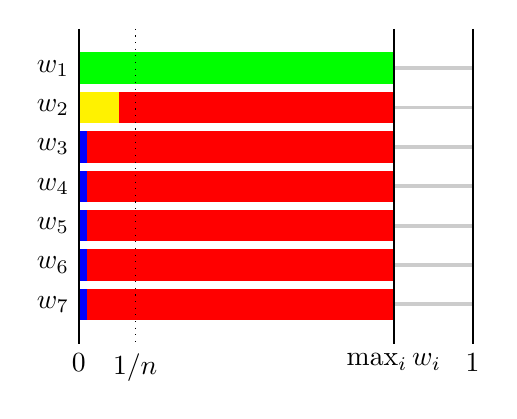
\begin{tikzpicture}
            \foreach \x/\c [count = \i] in {0.8/green, 0.1/yellow, 0.02/blue, 0.02/blue, 0.02/blue, 0.02/blue, 0.02/blue} {
            \node[anchor=west, minimum width=\w, minimum height=0.5mm, fill=black!20, inner sep=0] at (0mm, -\i * \h) {};
            \node[anchor=west, minimum width=\w*0.8, minimum height=4mm, fill=red, inner sep=0] at (0mm, -\i * \h) {};
            \node[anchor=west, minimum width=\w * \x, minimum height=4mm, fill=\c, inner sep=0, label=left:{$w_\i$}] at (0mm, -\i * \h) {};
            }

            \def\b{-8 * \h}

            \path[draw, thick] (0, 0) to ++(0, \b) node[below] {0};
            \path[draw, thick] (\w, 0) to ++(0, \b) node[below] {1};

            \path[draw, thick] (\w * 0.8, 0) to ++(0, \b) node[below] {$\max_i \set{w_i}$};
            \path[draw, dotted] (\w / 7, 0) to ++(0, \b) node[below] {$1/n$};
        \end{tikzpicture}
    \end{center}
    \caption{
        Rejection Sampling bei stark verzerrter Verteilung.
        Wir wählen zuerst eine Zeile zufällig uniform.
        Dann ziehen wir uniform zufällig einen horizontalen Punkt.
        Wenn wir dabei die rote Linie treffen verwerfen wir --- bei der gezeigten Verteilung in Zeilen $2$ bis $n$ also fast immer.
    }
    \label{fig:alias-tab-motivation}
\end{figure}

Eine vergleichbar problematische Situation ist in \cref{fig:alias-tab-motivation} visualisiert.
Dem gegenüber wäre eine besonders gute Eingabe ein $w_i = 1/n \pm \epsilon$ für alle $i$.
In der Abbildung würde das der Situation entsprechen, dass alle Zeilen etwa auf der gestrichelten Linien enden würden --- es käme zu keiner Rejection.

Tatsächlich können wir durch einen kleinen Kniff eine beliebige Eingabe komplett ohne Verwerfung samplen.
Hierzu beobachten wir, dass die Fläche der grünen Box von $w_1$ rechts des gestrichelten Durchschnitts genau der roten Fläche links des Durchschnitts entspricht.
Dies folgt, da sonst die gestrichelte Linie sonst nicht der Durchschnitt wäre.

Die Idee der Alias Methode besteht darin, die den Überschuss auf die rote Fläche aufzuteilen.
Hierbei wollen wir aber am \emph{entweder-oder} Schema der Verwurfsmethode festhalten;
sprich pro Zeile soll es nur zwei Wahlen geben.
Das ist problematisch, da es bis zu $n-1$ überlange Zeilen geben kann, die dann nicht alle in die eine unterlange Zeile verteilen dürfen.

Um im Folgenden nicht ständig den Durchschnitt $1/n$ als Faktor schreiben zu müssen, nehmen wir an, dass die Gewichtssumme~$\sum_i w'_i$ auf $n$ statt auf $1$ normiert ist.
Dann folgt das durchschnittliche Gewicht als $\sum_i w'_i / n = n /n = 1$.
Die Alias-Tabelle baut auf folgender Einsicht auf:

\begin{theorem}
    Seien $w_1, \ldots, w_n$ nicht-negative reelle Gewichte mit Summe $\sum_i w_i = n$.
    Dann können wir eine Tabelle mit $n$ Zeilen konstruieren, so dass jede Zeile ein Gewicht von genau $1$ hat, und höchstens zwei Einträge pro Zeile vorhanden sind.
\end{theorem}

\begin{proof}[Beweis durch Induktion]
    Für $n=1$ ist die Aussage trivial wahr, da es nur ein Gewicht $w_1 = 1$ gibt.
    Nehmen wir also an, dass die Aussage für $n$ gilt und betrachten $n + 1$.

    Wir haben also Gewichte $w_1, \ldots, w_{n+1}$ mit $\sum_{i=1}^{n+1} w_i = n + 1$.
    Dann existieren Indizes $k$ und~$g$ mit $w_k \le 1$ und $w_g \ge 1$ (beobachte, dass wir $k = g$ nicht ausschließen).
    Da $w_k \le 1$ müssen wir ein Gewicht $c = 1 - w_k$ ergänzen, um eine Zeile mit Gewicht $1$ zu erhalten.
    Dies nehmen wir uns von $w_g$ und produzieren die Zeile.

    Übrig bleiben alle unveränderten Gewichte $w_i$ mit $i \not\in \set{g, k}$.
    Falls $g = k$, war $w_k = 1$ und $c=0$.
    Falls $g \ne k$, verbleibt noch Eintrag $g$ mit Gewicht $w_g - c > 0$.
    In jedem Fall sind noch $n$ Gewichte mit einer Summe von $(n+1) - 1 = n$ im Spiel.
    Per Induktionsannahme können wir für diese eine entsprechende Tabelle konstruieren.
\end{proof}

Konkret besteht unsere Tabelle aus zwei Arrays $G[1\ldots n]$ und $A[1\ldots n]$.
In der $i$-ten Zeile speichern wir als ersten Eintrag Element~$i$ mit einem anteiligen Gewicht von $G[i] \le w_i$ ab.
Der Rest der Zeile wird vom sog. Alias $A[i]$ eingenommen, der per Konstruktion ein Gewicht $1 - G[i]$ hat und daher nicht explizit gespeichert werden muss.

Für jede endliche Verteilung $w_1, \ldots, w_n$ können wir eine solche Tabelle in Zeit $\Oh{n}$ konstruieren --- i.A. ist die Tabelle aber nicht eindeutig.
Eine mögliche Belegung kann mittels zweier Listen $K$ (kleiner) und $D$ (drübba) erzeugt werden.
\begin{itemize}
    \item Falls $w_i < 1$ fügen wir $(i, w_i)$ in $K$ ein
    \item Falls $w_i \ge 1$ fügen wir $(i, w_j)$ in $D$ ein
\end{itemize}

Solange $K$ und $D$ nicht leer sind, entnehmen wir ein Element $(k, w_k)$ aus $K$ und ein Element $(g, w_g)$ aus $D$.
Wir schreiben $G[i] = w_k$ und $A[i] = g$.
Sei $w'_g = w_g - (1 - w_k)$ das verbleibende Gewicht von $g$.
Wenn $w'_g < 1$ fügen wir $(g, w'_g)$ in $K$ ein, sonst in $D$.

Per Konstruktion kann $K$ niemals vor $D$ leer werden; es kann aber durchaus vorkommen, dass $K$ leer ist, während $D$ noch Werte enthält.
Dann haben aber alle Einträge in $G$ Gewicht genau $1$; wir können sie in der offensichtlichen Art in $G$ ein.
Praktische Implementierungen müssen aufgrund der wiederholten Subtraktionen mit Rundungsfehlern der Gewichte umgehen können;
dann kann auch $D$ zuerst leer werden; die Elemente in $K$ haben dann aber Gewicht $1 - \epsilon$.

Das Ziehen aus der Alias-Tabelle läuft analog zu Rejection-Sampling:
wir wählen eine Zeile $1 \le i \le n$ zufällig uniform und werden ein reelles $0 \le u \le 1$.
Falls $u < G[i]$ geben wir $i$ zurück, sonst $A[i]$.
Die gelingt in Zeit $\Oh{1}$.

\subsection{Intermezzo: Schnelles Ziehen von uniformen Ganzzahlen}
\emph{Dieses Kapitel basiert in auf \cite{DBLP:journals/tomacs/Lemire19}.}
Wir übernehmen auch die Notation $a \div b = \lfloor a / b \rfloor$.

\bigskip

Auf praktischen Computern erhalten wir (Pseudo)Zufallszahlen in der Regel in der Größe eines Maschinenwortes, oft mit $L = 32$ oder $64$ Bit.
Wir können dies entweder als $L$~unabhängige Zufallsbits interpretieren, oder z.B. als eine vorzeichenlose Ganzzahl~$X$, die uniform auf $[0, 2^L)$ verteilt ist.
In Anwendungen benötigen wir jedoch häufig Zahlen aus einem Intervall $[a, b)$ und müssen daher $X$ transformieren.

Den kleinsten Wert anzupassen ist einfach: wir ziehen aus $Y' \in [0, b-a)$ und geben $Y = a + Y'$ zurück.
Daher reduzieren wir im Folgenden die Diskussion auf Intervalle $[0, s)$, wobei wir $1 \le s \le 2^L$ annehmen (die obere Schranke lässt sich durch Konkatenation mehrerer $L$-Bit Wörter umgehen).

In der Praxis wird eine Zahl $X \in [0, 2^L)$ oft auf $[0, s)$ reduziert, indem $Y = X \bmod s$ berechnet wird
--- allein auf GitHub findet sich das Pattern \qq{\texttt{rand() \%}} fast eine halbe Millionen mal.
Der einzige Grund: es ist schnell zu schreiben und garantiert $Y \in [0, s)$.
Es ist aber zum einen recht langsam, und auch nur dann uniform, wenn $2^L \bmod s = 0$ gilt.
Dies lässt sich an einem Bild leicht erkennen.
Betrachte die Sequenz $0, \ldots, 2^L \bmod s$:

\begin{align}
    \underbrace{
        \overbrace{0, 1, \ldots, s{-}1}^\text{$s$ Werte},\ \
        \overbrace{0, 1, \ldots, s{-}1}^\text{$s$ Werte},\ \
        \ldots, \ \
        \overbrace{0, 1, \ldots, s{-}1}^\text{$s$ Werte}
    }_\text{$(2^L \div s)$ Blöcke mit insg. $2^L - (2^L \div s)$ Werten},\ \
    \overbrace{0, 1, \ldots, (2^L \bmod s){-}1}^\text{$2^L \bmod s$ Werte},\ \
    \label{eq:s_bloecke_in_2l}
\end{align}

Jeder Wert in $[0, s)$ taucht also exakt $\lfloor 2^L / s \rfloor$ oder $\lceil 2^L /s \rceil$ oft auf.
Es handelt sich also genau dann um eine uniforme Verteilung, wenn $\lfloor 2^L / s \rfloor = \lceil 2^L /s \rceil\ \ \Leftrightarrow\ \ 2^L \bmod s = 0$.
Wir formalisieren dies in folgendem Lemma:

\begin{lemma}\label{lem:gleichverteilt_in_ab}
    Seien $a < b$ die Grenzen des Intervalls $[a, b)$ und $s \in \mathbb N_{>0}$.
    Dann existieren für jedes $0 \le c < s$ genau dann $(b - a) \div s$ verschiedene Ganzzahlen $x \in [a, b)$ mit $x \bmod s = c$, wenn $s$ die Intervalllänge $b-a$ teilt.
\end{lemma}
\begin{proof}[Beweis durch Bild]
\end{proof}

Für $s \ll 2^L$ kann der Unterschied zwischen $\lfloor 2^L /s \rfloor$ und $\lceil 2^L / s \rceil$ verschmerzbar klein sein, für $s > 2^L / 2$ gibt es aber einige Elemente die mit doppelter Wahrscheinlichkeit von anderen zurück geliefert werden.

\subsubsection{Rejection Sampling to the help}
Es sollte nicht überraschen, dass Rejection Sampling hier helfen kann.
Ein naiver Ansatz verwirft $X \ge s$ und akzeptiert nur $X < s$.
Wenn $X$ uniform ist, ist es die Ausgabe dann auch.
Allerdings ist für $s \ll 2^L$ die Verwerfungsrate exorbitant hoch;
in Erwartung benötigen wir $2^L / s$ Versuche!

Besser ist es natürlich ein möglichst großes $k \ge 1$ zu wählen, s.d. $k s \le 2^L$.
Dann verwerfen wir nur $X \ge ks$ und liefern sonst $X / k$ zurückzuliefern.
Die beste Wahl ist $k = 2^L \div s$.
Dieses Verfahren hat eine Akzeptanzwahrscheinlichkeit von
\begin{align}
    \frac{k \cdot s}{2^L} = 1 - \frac{2^L \bmod s}{2^L} \ge 1/2,
\end{align}
und benötigt daher in Erwartung höchstens zwei Versuche.

Beobachte, dass es hierbei egal ist, ob wir $X \ge ks$ oder $X < (2^L - ks) = 2^L \bmod s = (2^L -s) \bmod s$ verwerfen.
Die letzte Variante ist aber auf echten Maschinen in der Regel schneller.
Das führt zu folgendem Schema, das auch als OpenBSD Algorithmus bekannt ist:

\begin{algorithm}[H]
    $t \gets (2^L - s) \bmod s$\tcc{$2^L \bmod s = (2^L -s) \bmod s$. $2^L$ ist aber ggf. ein Overflow}\;
    $x \gets \text{zufällige Ganzzahl aus $[0, 2^L)$}$\;
    \While{x < t}{
    $x \gets \text{zufällige Ganzzahl aus $[0, 2^L)$}$\;
    }
    \Return $x \bmod s$\;
    \caption{OpenBSD Algorithmus: Ziehen uniformer Ganzzahlen.}
\end{algorithm}

Der OpenBSD Algorithmus ist einfach und korrekt, hat aber einen enormen Nachteil in der Praxis:
Pro Aufruf muss ein Modulo und eine Division (das ist idR dieselbe CPU-Instruktion!) berechnet werden.
Eine \texttt{div} Instruktion gehört zu den teuersten skalaren Operationen\footnote{Sehr umfangreiche Benchmarks und Infos: \url{https://www.agner.org/optimize/instruction_tables.pdf}}, die CPUs unterstützen.
Im Vergleich zu einfacher Arithmetik (z.B. Addition) ist eine Division oft um ein bis zwei Größenordnungen langsamer.
Insb. erzeugen moderne nicht-kryptographischen Pseudozufallsgeneratoren eine Zufallszahl oft schneller als eine einzelne Division dauert!

OpenJDK verwendet ein anderes Verfahren, das die Anzahl der Division an die Anzahl der Runden des Rejection Samplings knüpft.

\begin{algorithm}[H]
    $x \gets \text{zufällige Ganzzahl aus $[0, 2^L)$}$\;
    $r \gets x \bmod s$\;
    \While{$x - r > 2^L - s$}{
    $x \gets \text{zufällige Ganzzahl aus $[0, 2^L)$}$\;
    $r \gets x \bmod s$\;
    }
    \Return $r$;
    \caption{Java Algorithmus zum Ziehen uniformer Zufallszahlen.}
\end{algorithm}

Wir müssen genau dann verwerfen, wenn $ks \le x \le (k+1)s$ mit $(k+1)s > 2^L$, d.h. wenn $x$ aus einem \qq{$s$-Intervall} stammt, das nicht vollständig in $[0, 2^L)$ enthalten ist.
Beobachte, dass $x - r = x - (x \bmod s) = (x \div s)s$ dem größten Vielfachen von $s$ entspricht, das $x$ nicht übersteigt;
es ist also die linke Intervallgrenze.
Die rechte Intervallgrenze ergibt sich dann als $x- r +s$.
Allerdings kann $x - r + s$ zu einem Überlauf führen; daher prüft der Algorithmus --äquivalent aber sicher vor Überlauf--- auf $x - r > 2^L - s$.

Der Vorteil von des Java-Algorithmus gegenüber der OpenBSD Methode besteht darin, dass Java im günstigen Fall nur eine Division ausführen muss.
Wenn für $s \to 2^L$ die Verwerfungsrate jedoch steigt, nimmt auch die Anzahl der Division zu und ist im Worst-Case gar unbeschränkt (eine WHP Schranke lässt sich mittels Chernoff zeigen).

Lemire~\cite{DBLP:journals/tomacs/Lemire19} schlägt daher ein Verfahren vor, das oft komplett ohne (generische) Division auskommt und im Worst-Case nur eine benötigt.
Hierzu nutzt er aus, dass eine Division $x \div 2^k$ nicht durch eine aufwendige \texttt{div} Instruktion ausgeführt werden muss, sondern einfach einem Bitshift um $k$ Bits nach rechts entspricht.
Konkret nutzen wir, dass
\begin{align}
    0 \ \le \ (x \cdot s) \div 2^L  <  s
    \quad \forall x \in [0, 2^L), s \in [0, 2^L)
\end{align}

Dabei implementieren wir $(x \cdot s) \div 2^L$ als $\texttt{shift-right}(x \cdot s, L)$; der Ausdruck ist also im Wesentlichen eine Multiplikation von zwei $L$-Bit Zahlen zu einer Zahl mit $2L$ Bit gefolgt von einem Shift um $L$ Bits.
Analog können wir die unteren $L$ Bits mittels Verundung der unteren $L$ Bits extrahieren.
Warum ist das nützlich?

Durch die Multiplikation von $s$ mit einem zufälligen $x \in [0, 2^L)$ bilden wir auf alle Vielfachen von $s$ in $[0, s\cdot 2^L)$ ab.
Durch die Division mit $2^L$, transformieren wir alle Vielfachen von $s$ in $[0, 2^L)$ auf $0$, in $[2^L, 2\cdot2^L)$ auf $1$, und $[i 2^L, (i+1)\cdot2^L)$ auf $i$.
Im Allgemeinen teilt aber $s$ nicht $2^L$ (sonst wären wir schon fertig);
daher müssen wir $2^L \bmod s$ Element aus dem Intervall herausschneiden.
Wir verwerfen daher für jedes $i$ die Elemente in $[i 2^L, i 2^L + (2^L \bmod s))$ und akzeptieren $[ i 2^L + (2^L \bmod s), (i+1)\cdot2^L)$.
Das führt zu folgendem Algorithmus:

\begin{algorithm}[H]
    $x \gets \text{zufällige Ganzzahl aus $[0, 2^L)$}$\;
    $m \gets x \times s$\;
    $\ell \gets m \bmod 2^L$\;
    \If(\tcc*{Abkürzung falls wir nicht sicher Akzeptieren können}){$\ell < s$}{
    $t \gets (2^L -s) \bmod s$\tcc*{$2^L \bmod s = (2^L -s) \bmod s$}
    \While{$\ell < t$}{
    $x \gets \text{zufällige Ganzzahl aus $[0, 2^L)$}$\;
    $m \gets x \times s$\;
    $\ell \gets m \bmod 2^L$\;
    }
    }
    \Return{$m \div 2^L$}
\end{algorithm}

Der \texttt{if}-Block ist dabei nicht funktional wichtig --- wenn wir die Bedingung durch \texttt{true} ersetzen, arbeitet der Algorithmus weiterhin korrekt und führt die Rejection richtig aus.
Er ist aber essentiell in der Vermeidung der Division.
Beobachte, dass $t = 2^L \bmod s = (2^L - s) \bmod s < s$ ist und wir nur verwerfen, wenn $\ell < t$.
Das bedeutet aber insbesondere auch, dass wir für $\ell \ge s$ wissen, dass $\ell$ nicht kleiner als $t$ sein kann.
Daher müssen wir $t$ erst gar nicht berechnen.
Der Algorithmus läuft daher nur mit Wahrscheinlichkeit $s / 2^L$ in den \texttt{true}-Block; mit der Gegenwahrscheinlichkeit $1 - s/2^L$ ist er also divisionsfrei.

Die Strategie Abkürzungen für sicheres Verwerfen/Akzeptieren zu konstruieren, um unnötige Berechnungen zu sparen, ist eine gängige Technik in effizienten Implementierungen von Rejection-Sampling.
